%\documentclass[a4paper,12pt]{article}
\documentclass[a4paper,12pt]{scrartcl}
\usepackage[usenames,dvipsnames]{color}

\usepackage{pgfplots, pgfplotstable}
\usepackage{fancyhdr}
\usepackage[utf8]{inputenc}				% encodage UTF-8
\usepackage[T1]{fontenc}
%\usepackage{fullpage}					% supprime marges
\usepackage[francais]{babel}
\usepackage{graphicx}
\usepackage{amsmath}
\usepackage{amssymb}
\usepackage{sectsty}
\usepackage{enumerate}
\usepackage{float}
\usepackage{listings}
\usepackage{listingsutf8}				% package PAS PAR DEFAUT + ? \usepackage{textcomp}


\usepackage[colorlinks=true, urlcolor=MidnightBlue, linkcolor=Black]{hyperref}

\lstset{
	tabsize=4,
	frame=single,
	breaklines=true,
	basicstyle=\ttfamily\small,
	frameround={tttt},
	showstringspaces=false,
	language=C,
	keywordstyle=\color{blue},
	commentstyle=\color{OliveGreen},
	stringstyle=\color{red}\itshape,
	inputencoding=utf8/latin1,
}

\pagestyle{fancy}
\setkomafont{disposition}{\normalfont\bfseries}

\lfoot{}
\cfoot{Commission Championnats de France 2017}
\rfoot{\thepage}
\renewcommand{\headrulewidth}{0.0pt}
\renewcommand{\footrulewidth}{0.4pt}
%\renewcommand{\chaptermark}[1]{ \markboth{#1}{} }
\renewcommand{\sectionmark}[1]{ \markright{#1}{} }

%\fancyhead[R]{\textit{\nouppercase{\rightmark}} }
\fancyhead[R]{}
\fancyhead[CL]{}
%\fancyhead[LO]{\textit{\nouppercase{\rightmark}} }

%\textwidth 16cm
\textheight 24cm
\hoffset 0mm
\voffset 0.5cm

\sectionfont{
    \sectionrule{0pt}{0pt}{-5pt}{0.8pt}
}



%===============
\begin{document}
%===============

\begin{titlepage}
    \centering
    \vfill
    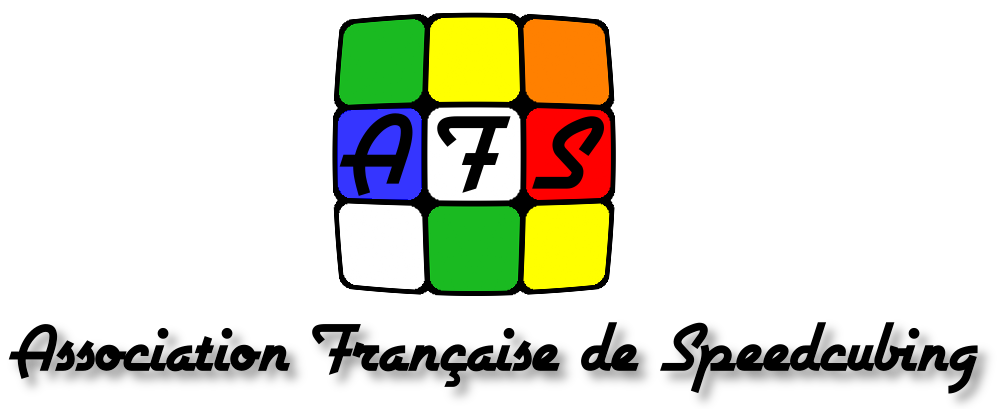
\includegraphics[width=\textwidth]{logoafsletters.png}
    \vfill
    {\bfseries\Huge
        Organisation des championnats de France 2017\\
	\large
        Document destiné aux équipes d'organisation candidates\\
        \vskip2cm
        Kévin Cagnon, Victor Colin, Philippe Virouleau\\
        \vskip1cm
	13 Mars 2016
    }    
    \vfill
\end{titlepage}


\pagebreak
%~
%\newline

%---------
%	Introduction
%---------

\section*{Préambule}

Ce document est destiné aux équipes candidates à l'organisation des championnats de France
de Rubik's cube 2017.

La première partie présente les modalités de candidature et le contenu attendu de celle-ci.

La seconde donne une idée des critères de sélection que la commission va utiliser
pour départager les candidats. Elle décrit les attentes de la commission concernant
le dossier déposé. Elle contient également des conseils sur les points importants des candidatures.


\section*{Dépot des candidatures}

Vous avez jusqu'au 27 Avril pour déposer vos dossiers de candidature pour l'organisation
des championnats de France 2017. Le dépôt se fait auprès de la commission des championnats
de France, à l'adresse \href{mailto:cdf@speedcubingfrance.org}{cdf@speedcubingfrance.org}.
Le format privilégié est le pdf ;
si votre dossier contient d'autres détails qui ne seraient pas communicables au format
pdf, merci de réaliser une archive (zip ou tar) contenant tout ce que vous souhaitez
nous faire parvenir.
Aucun dossier comprenant un membre de la commission dans son équipe d'organisation ne 
sera accepté.

Note : la date limite a été volontairement mise très tôt afin, idéalement, de
pouvoir annoncer le lieu pendant les championnats de France 2016. Nous ne souhaitons
en aucun cas pénaliser une équipe d'organisation qui serait en manque de temps :
si vous avez un projet sérieux mais que le délai pour déposer le dossier n'est pas
suffisant, merci de contacter dès maintenant la commission, afin d'envisager un
rallongement de la période de dépôt. Néanmoins nous ne dépasserons pas le 13 Août comme dernier délai
pour le dépôt de dossier.

Nous espérons que les équipes d'organisation susceptibles d'être candidates ont
déjà une idée de projet et qu'il ne reste plus qu'à rédiger le dossier, ce pour
quoi le délai accordé devrait être suffisant.

\pagebreak
\section*{Évaluation des candidatures}

Cette partie décrit les attentes de la commission concernant les dossiers de candidature.
Il contient certains impératifs, des indications sur les points importants que la
commission étudiera, mais aussi des informations et conseils variés, basés sur
notre expérience et les éditions précédentes.  Il n’est pas attendu que tous
les points soient respectés à la perfection, mais que le dossier soit, d’une
manière générale, digne d’une candidature pour une compétition de cette importance.

Une fois que la commission aura rendu sa décision, il est impératif que l'équipe
d'organisation annonce les caractéristiques majeures du projet (telles que la date
et le lieu), dans un délai d'un mois.

\subsection*{Équipe d’organisation}


La commission prendra en compte la taille et l’expérience de l’équipe d’organisation, il faudra être le plus explicite possible sur les rôles de chacun au sein de l’équipe. Afin d’éviter les quiproquos, merci d’indiquer les id WCA des membres.


\subsection*{Date}

Pour des raisons historiques, ainsi que pour faciliter le \emph{sponsoring} des gagnants au prochain championnat majeur le cas échéant, il reste préférable, dans la mesure du possible, que les Championnats de France se déroulent un week end entre fin mars et début mai 2017.


\subsection*{Lieu}


L’accessibilité de la ville accueillante est un critère primordial. Les compétiteurs arrivent de la France entière, éventuellement de l’étranger, et doivent pouvoir se rendre dans la ville par les transports en commun, notamment.


La salle doit être suffisamment grande pour accueillir tous les compétiteurs confortablement.
En fonction de la ville hôte, l’affluence peut varier de 75 à 150 personnes. 
\href{https://www.worldcubeassociation.org/regulations/translations/french/#article-7-environment}{Le règlement de la WCA impose de nombreuses contraintes sur le lieu d'accueil}.
Entre autre une zone de mélange séparée de la zone de compétition, ainsi qu’une zone d’attente, elle aussi séparée, sont requises afin de réduire les risques de triche.
La salle devra également être correctement éclairée, en particulier la zone de compétition, et la température devra être adéquate pour permettre à tout le monde de concourir dans les meilleures conditions.

\subsection*{Site Internet}


Le site Internet de la compétition devra proposer une version anglaise, afin que
les étrangers souhaitant participer puissent avoir toutes les informations.
Dans la mesure du possible il devra être clair et complet. Des membres de la
commission peuvent vous aider sur ce point, et si besoin l'AFS peut servir
d'hébergeur pour le site internet.

\subsection*{Planning}

Hormis la présence de l’intégralité des épreuves officielles, aucun impératif n’est donné.
Cependant, la commission se réserve le droit de proposer des modifications sur le
nombre de tours par épreuve ainsi que les time limits envisagées

Le planning définitif n’est pas demandé, mais une ébauche complète est indispensable :
épreuves prévues, \emph{time limits} et \emph{cutoffs} éventuels pour chaque
épreuve, nombre de tours et de qualifiés pour chaque épreuve, répartition du
tout sur la durée de la compétition. L’épreuve reine étant le Rubik’s Cube 3x3x3,
il est vivement conseillé d’en proposer 3 tours et sans modification de la
\emph{time limit} par défaut (10 minutes), afin qu'un maximum de personnes puisse
y prendre part.














\subsection*{Budget}


Le budget dépendra principalement de vos sponsors et subventions, vous êtes libre de sa répartition.

Notez tout de même que certains sponsors refusent d'êtres associés à d'autres et qu'il
faut donc être vigilant quant à leur choix. La commission peut cependant vous donner
les pistes suivantes :

\begin{itemize}
    \item Démarcher les conseils généraux, les instances locales, les comités départementaux
	olympiques et sportifs.
    \item Démarcher les entreprises locales en leur faisant par la suite un peu de
	publicité peut être une solution très intéressante.
    \item \emph{Kingscube} est un sponsor avec qui les cubeurs ont des contacts
	privilégiés et pouvant fournir des lots (les détails sont à négocier en
	fonction de votre partenariat).
    \item Enfin, sachez que \emph{7 Towns} pourra être contacté pour obtenir des médailles
	si vous le souhaitez (à notre connaissance ils n'ont jamais refusé d'en envoyer
	si la demande leur est faite suffisamment à l'avance).
\end{itemize}



Cas particulier : \emph{Winning Moves} a été l'initiateur du Championnat de France
depuis 2003. En 2013, l’entreprise a arrêté de proposer le championnat, et a donc
laissé la communauté s’en occuper. 
Pour cette première édition organisée par la communauté, \emph{Winning Moves} a été le financeur principal,
néanmoins depuis 2013 Thierry Karpiel a quitté \emph{Winning Moves} pour fonder \emph{Win Games}.
Si l'intérêt de \emph{Win Games} pour le \emph{sponsoring} des championnats de France
semble avoir grandement diminué, il devrait toujours être possible de les contacter.  

Ces points ne sont que des pistes de réflexion pour vous permettre de mettre en place
votre dossier, vous restez libre de choisir les sponsors que vous souhaitez.


\subsection*{Prix et récompenses}


Plusieurs types de prix et récompenses sont possibles. Les éditions précédentes ont
notamment proposé des prix sous forme d’argent, des lots pour les podiums,
des invitations aux championnats internationaux, des remboursements du trajet aux
Championnats de France pour les \emph{subX} ou les \emph{N} premiers.

Afin de rendre les Championnats de France attractifs et accessibles pour le plus
grand nombre, il sera apprécié qu’une partie du budget “lots” soit consacrée au
remboursement des trajets, dans les limites de votre choix.


\subsection*{Dispositions supplémentaires}


Aucune disposition supplémentaire n’est requise, cependant un partenariat pour le
logement, le transport ou la restauration par exemple, sera un plus.
Bien entendu, la réalisation d’idées nouvelles, originales, ou attendues par la
communauté, sera sûrement appréciée !

\section*{Informations complémentaires}

Il nous semble important que vous sachiez à qui vous vous adressez ; la commission
est composée des 3 membres suivants :

\begin{itemize}
    \item Kévin Cagnon (\href{https://www.worldcubeassociation.org/results/p.php?i=2014CAGN01}{2014CAGN01})
    \item Victor Colin (\href{https://www.worldcubeassociation.org/results/p.php?i=2013COLI02}{2013COLI02})
    \item Philppe Virouleau (\href{https://www.worldcubeassociation.org/results/p.php?i=2008VIRO01}{2008VIRO01})
\end{itemize}

Nous avons tous organisé et participé à de multiples compétitions, et nous utiliserons notre
expérience pour choisir le meilleur candidat parmi les dossiers soumis. De plus,
au-delà du choix du dossier retenu pour l'édition 2016 des championnats de France,
nous sommes également là pour vous conseiller si vous en avez besoin. N'hésitez
donc surtout pas à prendre contact avec nous à l'adresse
\href{mailto:cdf@speedcubingfrance.org}{cdf@speedcubingfrance.org}.





%=============	
\end{document}
%=============
